\section{Transformer - Run-time Reconfigurable Heterogeneous Architecture}
\label{sec_arch}


\subsection{Architecture Overview}

Figure \ref{fig_arch} shows {\em Transformer}, heterogeneous
architecture for transparent acceleration of dynamic
workloads. Transformer consists of cores with private L1 caches, and a
partial reconfigurable logic unit ( also called programmable
accelerator in this paper) for instantiating acceleration
functions. The reconfigurable logic, equipped with input and output
buffers, shares the L2 cache with the cores through dedicated DMA
channels. All processing elements (cores and accelerator) are
interconnected via a mesh-type network on chip (NoC). The memory
hierarchy (private memory units of both cores and the accelerator,
shared L2 cache and main memory) follows MOESI protocol to maintain
coherence.

\begin{figure}
    \centering
    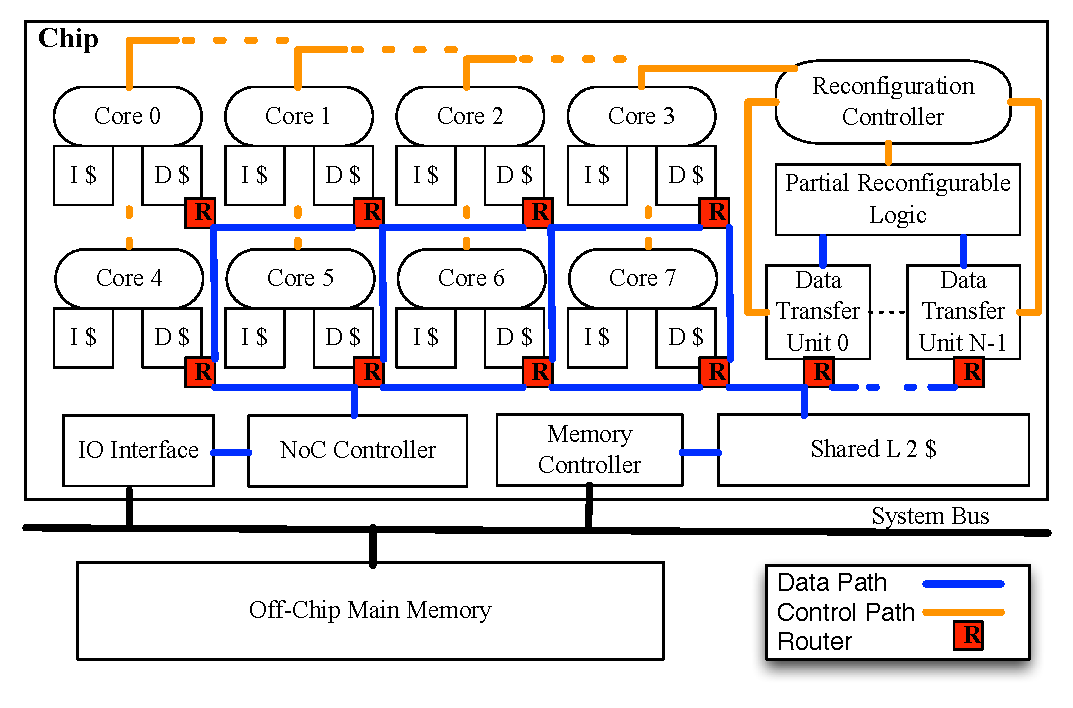
\includegraphics[width=4.0 in]{HPCA14-arch}
    \caption{Architecture Overview of {\em Transformer} }
    \label{fig_arch}
\vspace{-0.05in}
\end{figure}

Transformer's reconfigurable logic consists of computational resources
and {\em N} data transfer
units, supporting the instantiation of {\em N} independent accelerator
functions. The computational resources are organized in BRAM, DSP,
SLICEs as in a generic FPGA chip. The actual number of functions instantiated in the
programmable logic depends on the particular functions selected to
speed up at runtime and the resource requirements of the hardware
implementation of these functions. We study the architectural tradeoffs of 
reconfigurable logic and the number of cores in terms of performance
gains and power savings in Section \ref{sec_perf}.

Figure \ref{fig_reconfig_controller} depicts the three key components
in controlling the reconfiguration of accelerator logic:
reconfiguration controller, reconfigurable logic and data transfer
units. The reconfiguration controller is responsible for programming
new functions into the reconfigurable logic through new bit streams or
partial reconfiguration. Using control/status registers to record the
status of the reconfiguration logic, the controller receives
instructions from the middleware running on one of the cores, tracks
demands to various function calls, and makes decisions on what and
when to accelerate function(s).

The reconfigurable logic consists of a static region, a Partial
Reconfigurable Region (PRR) and an Internal Configuration Access Port
(ICAP). The static region contains necessary logic other than the
accelerator PRMs, such as clock module, interconnection interface and
memory control interface. The PRR can be divided into smaller
sub-regions and configured with different partial bit streams on
demand. ICAP is notified by the reconfiguration controller on what
kind of accelerator 
%PRMs ({\bf FIXME all different PRMs are located in
%  their fixed addresses}) 
should be configured and when to start. As a response, ICAP notifies
the controller about "resource full" and "(re)configuration done" by
writing to the specific bits of the control registers.

Each data transfer unit includes a pair of input and output buffers
that can be filled or drained by a DMA engine. The DMA engine is
responsible for bulk data transfer between the L2 cache and the
input/output buffers which are used as scratchpad memory for the
reconfigurable logic to complete necessary operations on the data. The
parameters such as memory addresses and data size of the DMA
operations are passed from the reconfiguration controller. TLB on each
of the data transfer unit is responsible for translating virtual
memory addresses to physical ones.


\begin{figure}
    \centering
    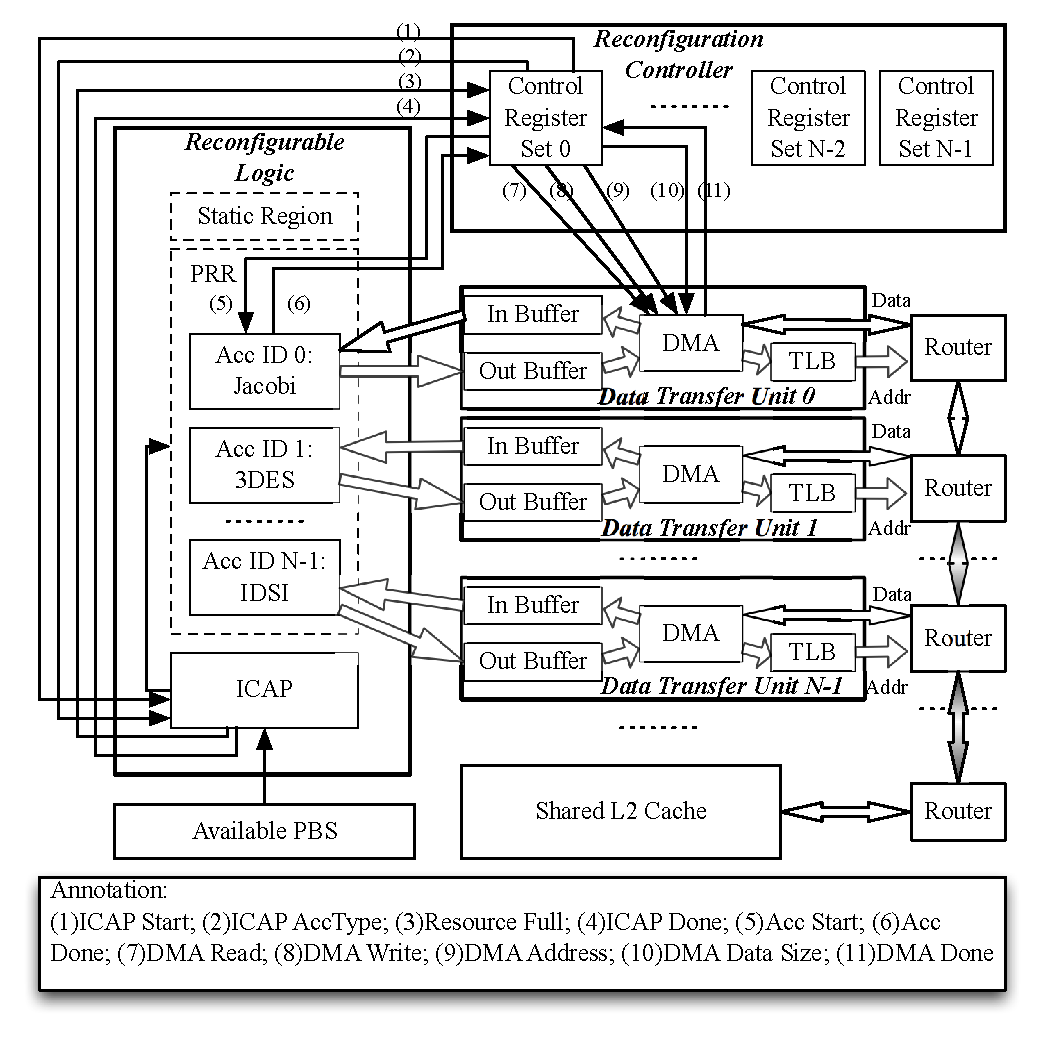
\includegraphics[width=4.0 in]{HPCA14-Controller}
    \caption{Transformer's Reconfigurable Logics and Controller}
    \label{fig_reconfig_controller}
\vspace{-0.05in}
\end{figure}


\subsection{Accelerator Invocation}

The invocation of accelerator from the software execution on a core is
done with specific accelerator instructions and control/status
registers. We illustrate how the accelerator is invoked in Figure
\ref{fig_Acc_Invoc}. We introduce {\em N} control register sets for
each to-be-instantiated accelerator and two new instructions to
invoke core-to-accelerator and accelerator-to-core execution path
transition. Each control register set contains three 32-bit registers:
general control register, DMA read register and DMA write
register. The general control register is responsible for ICAP control,
acceleration control and DMA control. The DMA read/write registers
contain read/write address of DMA operation source/destination
address. The specifications of the registers are described in Table
\ref{tbl_AccReg} and the two new instructions are listed as follows.

\begin{enumerate}
\item{\em readreg n}: read control register set with ID n.
\item{\em writereg n}: write the value into control register set with ID n.
%\item{\em accload AccReg n}: start configuring the type of accelerator
%  bitstream indicated by AccReg n into the reconfigurable logic. 
\end{enumerate}

\begin{table}[ht]
\scriptsize
\begin{center}
\begin{tabular}{|l|l|l|}
\hline 
\textbf{Register Name} & \textbf{Bits} & \textbf{Function}\\ 
\hline 
\hline
General Control &{\em Bit 0}   & ICAP start bit (IS)\\ 
\hline 
 &{\em Bit 1}   &  ICAP done bit (ID)\\ 
\hline 
 &{\em Bit 2-6} & ICAP accelerator type (IT 0-4)\\ 
\hline 
 &{\em Bit 7}   & acceleration start bit (AS)\\ 
\hline 
 &{\em Bit 8}   & acceleration done bit (AD)\\ 
\hline 
 &{\em Bit 9}   & DMA read enable (RE)\\ 
\hline 
 &{\em Bit 10}  & DMA write enable (WE)\\ 
\hline 
 &{\em Bit 11}  & DMA done (DD)\\
\hline
 &{\em Bit 12-15} & accelerator ID (ID 0-3)\\
\hline
 &{\em Bit 16-31} & DMA data block size (DS 0-15)\\
\hline
DMA Read Control &{\em Bit 0-31}  & DMA read address (RA 0-31)\\
\hline
DMA Write Control &{\em Bit 0-31} & DMA write address (WA 0-3)\\
\hline
\end{tabular} 
\caption{Control Registers for Reprogramming Accelerators.}
\label{tbl_AccReg}
\end{center}
\end{table}

The following is a brief introduction on how accelerator invocation
works. Note that all the set and reset operations are done by using
{\em readreg} and {\em writereg} instructions. These instructions are
encapsulated in customized wrapper functions, instead of being
directly used user applications.

\begin{enumerate}
\item If the reconfigurable controller decides to configure a specific
  combination of functions with the knowledge from middleware, the
  middleware will set the ICAP Start (IS) bit to start the
  reconfiguration process with the functions identified by ICAP
  accelerator type (IT 0-4) (This loading process will be skipped if
  the function is already configured in the accelerator logic.) At the
  same time, the middleware will prepare the data address and data
  block size by writing the DMA read address (RA 0-31) bits and DMA
  data block size (DS 0-15) bits.

\item Along with the reconfiguration process, we set the DMA Start
  (DS) bit to start reading the data from shared L2 cache or main
  memory into accelerator local input buffer until the buffer is full.

\item When the reconfiguration is done, ICAP will set the ICAP Done
  (ID) bit to enable the start of acceleration. By setting
  acceleration start (AS) bit, the Reconfiguration Controller causes a
  thread context switch on the corresponding core, which begins the
  execution of a different thread. The suspended thread will sleep
  until the acceleration done (AD) bit is set.

\item When the acceleration function is completed or the middleware
  decides to erase/change the accelerator function for the core,
  AccDone (AD) bit will be set and an interrupt will be generated to
  wake up the thread. Then the core will resume the previously
  sleeping thread, which will either continue a software path or get
  ready for the next accelerator invocation.
\end{enumerate}


\begin{figure}
    \centering
    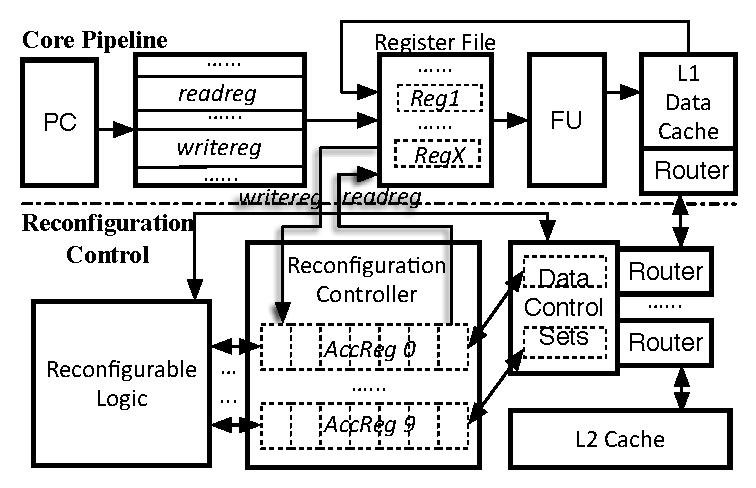
\includegraphics[width=4.0 in]{HPCA14-Acceleration_Invocation}
    \caption{Acceleration Invocation.}
    \label{fig_Acc_Invoc}
\end{figure}


To reduce the data transaction time from/to accelerators, a
combination of DMA and double buffering is used. 
Using double buffering, the accelerators can work on data residing in
their local memory while the DMA is fetching the next batch of data. A
TLB is located in between DMA and L2 cache to perform
virtual-to-physical address translation. This mechanism simplifies the
accelerator design, and guarantees the process isolation.
